% Figure 5.4 (Session 5): tensors as dots with legs, and the matrix product operator.
% The image is rendered by figures/blender/s5_4_tensor_notation.py; the coordinates of the labels
% come from figures/blender/out/tensor_notation_anchors.tex. Built by figures/blender/build_figure.sh.
\documentclass[11pt,tikz,border=0pt]{standalone}
\usepackage{amsmath,amssymb,graphicx,braket}
\usepackage{xcolor}
\definecolor{coursedark}{HTML}{1B2A4A}
\definecolor{costamber}{HTML}{B8620A}
\definecolor{sviolet}{HTML}{6A3FC8}
\newlength{\figw}\setlength{\figw}{16.19cm}   % the text width of the notes (letter, 2.7 cm margins), so labels print at size

\begin{document}
\begin{tikzpicture}[lbl/.style={font=\small, text=coursedark}]
  \node[anchor=south west, inner sep=0pt] at (0,0)
    {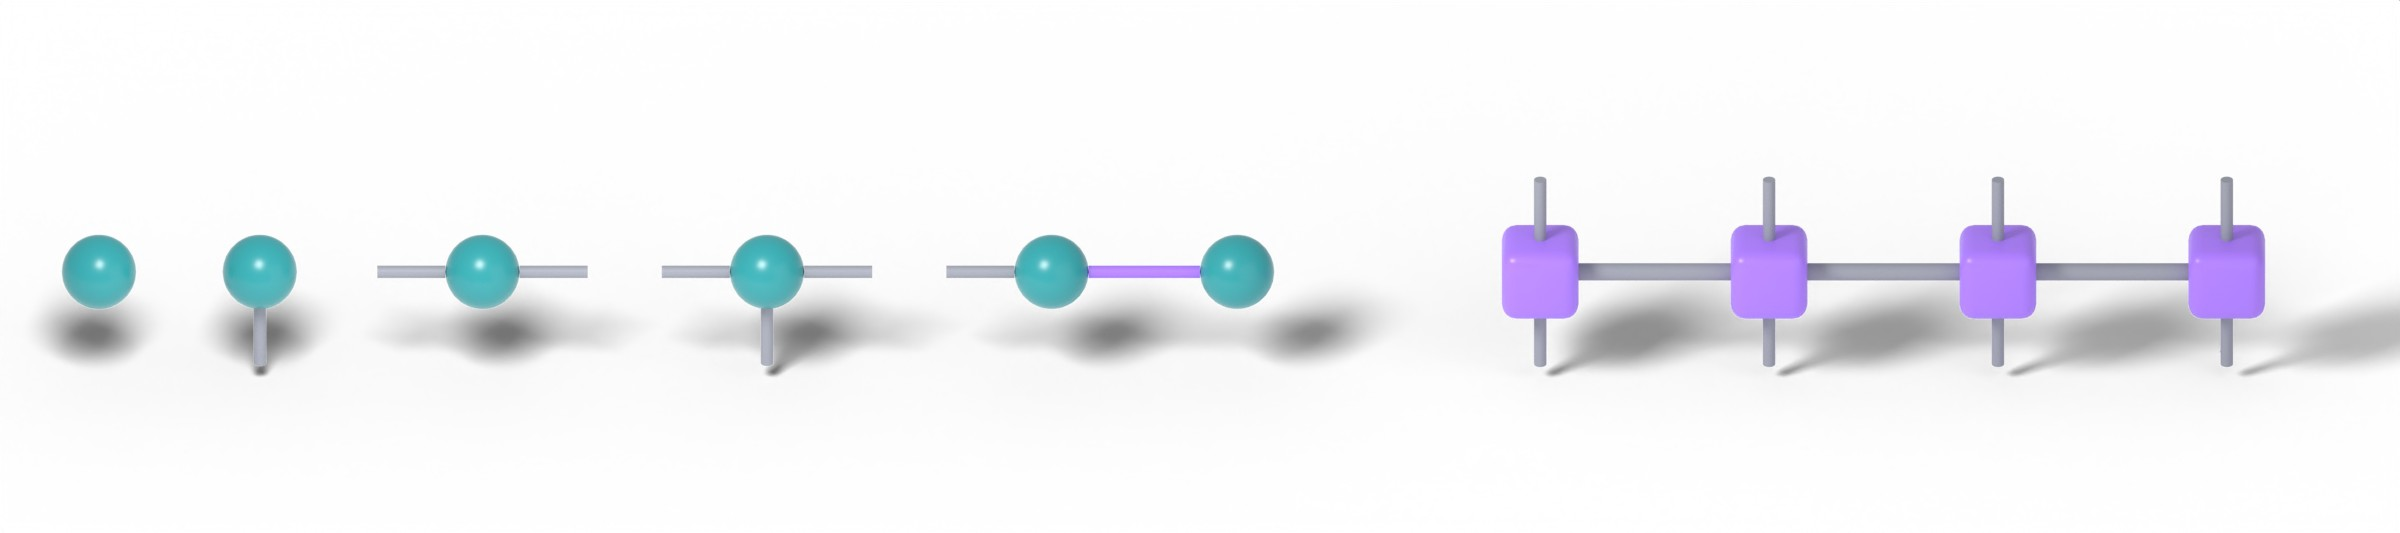
\includegraphics[width=\figw]{../blender/out/tensor_notation.jpg}};
  %% written by figlib.py; x and y in units of the image width
\coordinate (n0) at (0.0412\figw,0.0642\figw);
\coordinate (n1) at (0.1082\figw,0.0642\figw);
\coordinate (n2) at (0.2010\figw,0.0642\figw);
\coordinate (n3) at (0.3196\figw,0.0642\figw);
\coordinate (sum) at (0.4768\figw,0.0642\figw);
\coordinate (shared) at (0.4768\figw,0.1142\figw);
\coordinate (a) at (0.0206\figw,0.1780\figw);
\coordinate (Wlbl) at (0.7201\figw,0.1035\figw);
\coordinate (sup) at (0.7371\figw,0.1472\figw);
\coordinate (sdn) at (0.7371\figw,0.0704\figw);
\coordinate (chiW) at (0.8802\figw,0.1142\figw);
\coordinate (b) at (0.5902\figw,0.1780\figw);

  \node[lbl, font=\normalsize, anchor=west] at (a) {(a)};
  \node[lbl, font=\normalsize, anchor=west] at (b) {(b)};
  \node[lbl, anchor=north] at (n0) {$s$};
  \node[lbl, anchor=north] at (n1) {$v_i$};
  \node[lbl, anchor=north] at (n2) {$A_{ij}$};
  \node[lbl, anchor=north] at (n3) {$T_{ijk}$};
  \node[lbl, anchor=north] at (sum) {$\sum_j A_{ij}v_j$};
  \node[lbl, text=sviolet, anchor=south] at (shared) {$j$};
  \node[lbl, anchor=north east] at (Wlbl) {$W_i^{s_is_i'}$};
  \node[lbl, anchor=south] at (sup) {$s_i$};
  \node[lbl, anchor=north] at (sdn) {$s_i'$};
  \node[lbl, anchor=south] at (chiW) {$\chi_W$};
\end{tikzpicture}
\end{document}
